\addchap{ZIH}

%TODO: lustige Bildchen/Cliparts (höhö) um alles aufzulockern?

Das \textit{Zentrum für Informationsdienste und Hochleistungsrechnen} ist eine zentrale Einrichtung nicht nur unserer Fakultät, sondern der gesamten TU Dresden und ist für die gesamte Serverinfrastruktur und diverse technische Dienste verantwortlich. Vom ZIH werden dir ein paar sehr hilfreiche und relevante Dienste bereitgestellt, u.a. gehören dazu dein Login, dein E-Mail Account und das WiFi auf dem Campus.

Detailreiche Informationen zu den Services und deren Nutzung findest du auf dem ZIH Flyer, den du mit deinem Immatrikulationsbogen erhalten hast und auf der Seite des ZIH.
%\url{tu-dresden.de/zih/ese}. Wie genau machen wir das jetzt eigentlich mit den Links? Fortlaufende Nummern, die dann auf einer Linkseite hinten und/oder per Shortlink über unsere Seite irgendwie zugänglich sind? Beides zusammen wäre sicher nicht falsch.

\minisec{E-Mail}
Du bekommst vom ZIH zwei E-Mail Adressen:
\textit{s1234567@mail.zih.tu-dresden.de} und einen Alias von der Form \textit{vorname.nachname@mailbox.tu-dresden.de}.
Falls dein Name an der TU Dresden bereits existiert, lautet die Alias-Adresse für Max Mustermann dann z.B. \textit{max.mustermann1@mailbox...}.
Per Webmail oder IMAP kannst du auf dein Postfach zugreifen.
Alternativ kannst du deine Mails an eine persönliche Adresse weiterleiten, damit du nichts verpasst.
Vor allem wichtige E-Mails von der Uni werden an diese Adressen geschickt.

\minisec{WLAN}
Sowohl auf dem Campus wie auch in den Räumlichkeiten der Fakultät kannst du mit deinen Geräten ins Internet.
Das Netzwerk heißt \textit{eduroam} und bietet dir neben einem sicheren Internetzugang an unserer Uni selbes auch an sehr vielen anderen Universitäten weltweit. 
Zugang bekommst du mit deinem Login \textit{sXXXXXXX@tu-dresden.de} und deinem Passwort. Mehr Informationen findest du unter \link{NONE}.

\begin{figure}[h!]
\centering 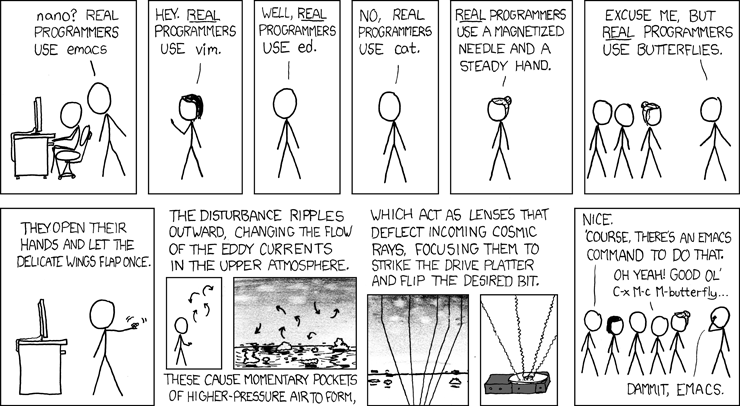
\includegraphics[width=\linewidth]{img/xkcd/real_programmers.png}
\caption*{{\small \textit{Real programmers set the universal constants at the start such that the universe evolves to contain the disk with the data they want. (xkcd/378)}}}
\end{figure}
%Bildlink: http://xkcd.com/378
